\documentclass[10pt, twocolumn]{article} 
\usepackage{simpleConference}
\usepackage{times}
\usepackage{graphicx}
\usepackage{amssymb}
\usepackage{url,hyperref}
\usepackage{mathtools}
\usepackage{algorithm}
\usepackage[noend]{algpseudocode}
\graphicspath{{./figures/}}


\begin{document}

\title{Real-time 3D Reconstruction at Scale Using VoxelHashing}

\author{Conner Brooks\\
\\
COT 4810\\
\today \\
\\
University of Central Florida\\
Orlando, FL, USA\\
\\
cbrooks@cs.ucf.edu\\
}

\maketitle
\thispagestyle{empty}


\begin{abstract}
The paper Real-time 3D Reconstruction at Scale using Voxel Hashing
\cite{niessner2013hashing} presents a new SLAM---Simultaneous Localization and
Mapping---system capable of producing high quality
reconstructions of a 3 dimensional environment with a low cost RGB-D sensor e.g.
the Microsoft Kinect. 
The novel contribution of this paper is a spatial hashing scheme that compresses space, allows for real-time access, and updates of surface data, all without the need for a regular or hierarchical grid data structure.
In this paper the initial implementation of KinectFusion \cite{izadi11}
\cite{newcombe11} will be described, as well as the spatial hashing approach
outlined in the paper by Nie{\ss}ner et al.
  
\end{abstract}



\section{Introduction}
3D reconstruction of environments is an important problem for robotics, virtual
reality, and augmented reality. Understanding the geometry allows a robot to
avoid obticals and navigate, and with augmented reality allows for interesting
interactions with the environment. The advent of commodity depth sensors has
resulted in a large amount of research concerning 3D understanding of
environments. This technology has been leveraged in the new Microsoft HoloLens \cite{hololens} which is a new head mounted augmented reality system.

The purpose of these systems and their development are to provide a dense 3D
mesh of the physical environment some agent---a robot or human---may be
positioned in. 
These systems allow for full 6 degrees of freedom (6DOF) tracking of where the agent is, and where it is looking, in the environment---that is the agent's translation $(x, y, z)$ cartesian coordinates in space (with respect to some origin, normally where the scan begins) and rotation or where the agent is pointed. 
This is similar to previous SLAM systems, however the difference is that the map created by this system is a dense mesh which is useful especially in augmented reality applications where we want to know where a surface is in order to place a virtual object or display an interface with respect to the environment. 
The difficulty with these application is normally tracking the pose of the user,
as it is slow and not robust enough for a common user to make efficient use of
the system; The extensions presented by Nie{\ss}ner et. al. provide a system
that improves the system to be robust enough such that a common user can scan
and move through the environment. 

The work by Nie{\ss}ner et al. can be seen as the state of the art
for large scale 3D reconstruction. To understand the work presented in this
paper, one must first understand the work in the seminal paper by Newcombe et
al. \cite{newcombe11}. This paper will begin with the basics of the KinectFusion
sytem an subsequently explain the novel approach taken by Nie{\ss}ner et al. \cite{niessner2013hashing}.

The open-source community has made some contributions to this
field, providing a few different implementations of the initial KinectFusion
algorithm as well as some of the extensions presented in this paper. A general
overview of these implementations will be provided in section
\ref{sec:opensource}. These implementations provide a good starting point for
someone who may want to extend upon the work presented here. The source code for
the implementation presented in this paper is available on github \cite{voxelhashing}.

\section{KinectFusion Overview}
The following is an overview of the KinectFusion system presented by Newcombe et
al. \cite{newcombe11} and Izadi et al. \cite{izadi11}.

\subsection{Understanding Depth Sensors}
This system takes as input multiple 2D depth images---also known as depth maps---and fuses them into a mesh. These depth maps are like normal 2D images but rather than each pixel storing a red, green, and blue value they store a single depth value, this depth image can be thought of as a 2D array or matrix of depth values. An example of this is shown in figure \ref{fig:depthimage}. 

\begin{figure}[h!]
  \centering
  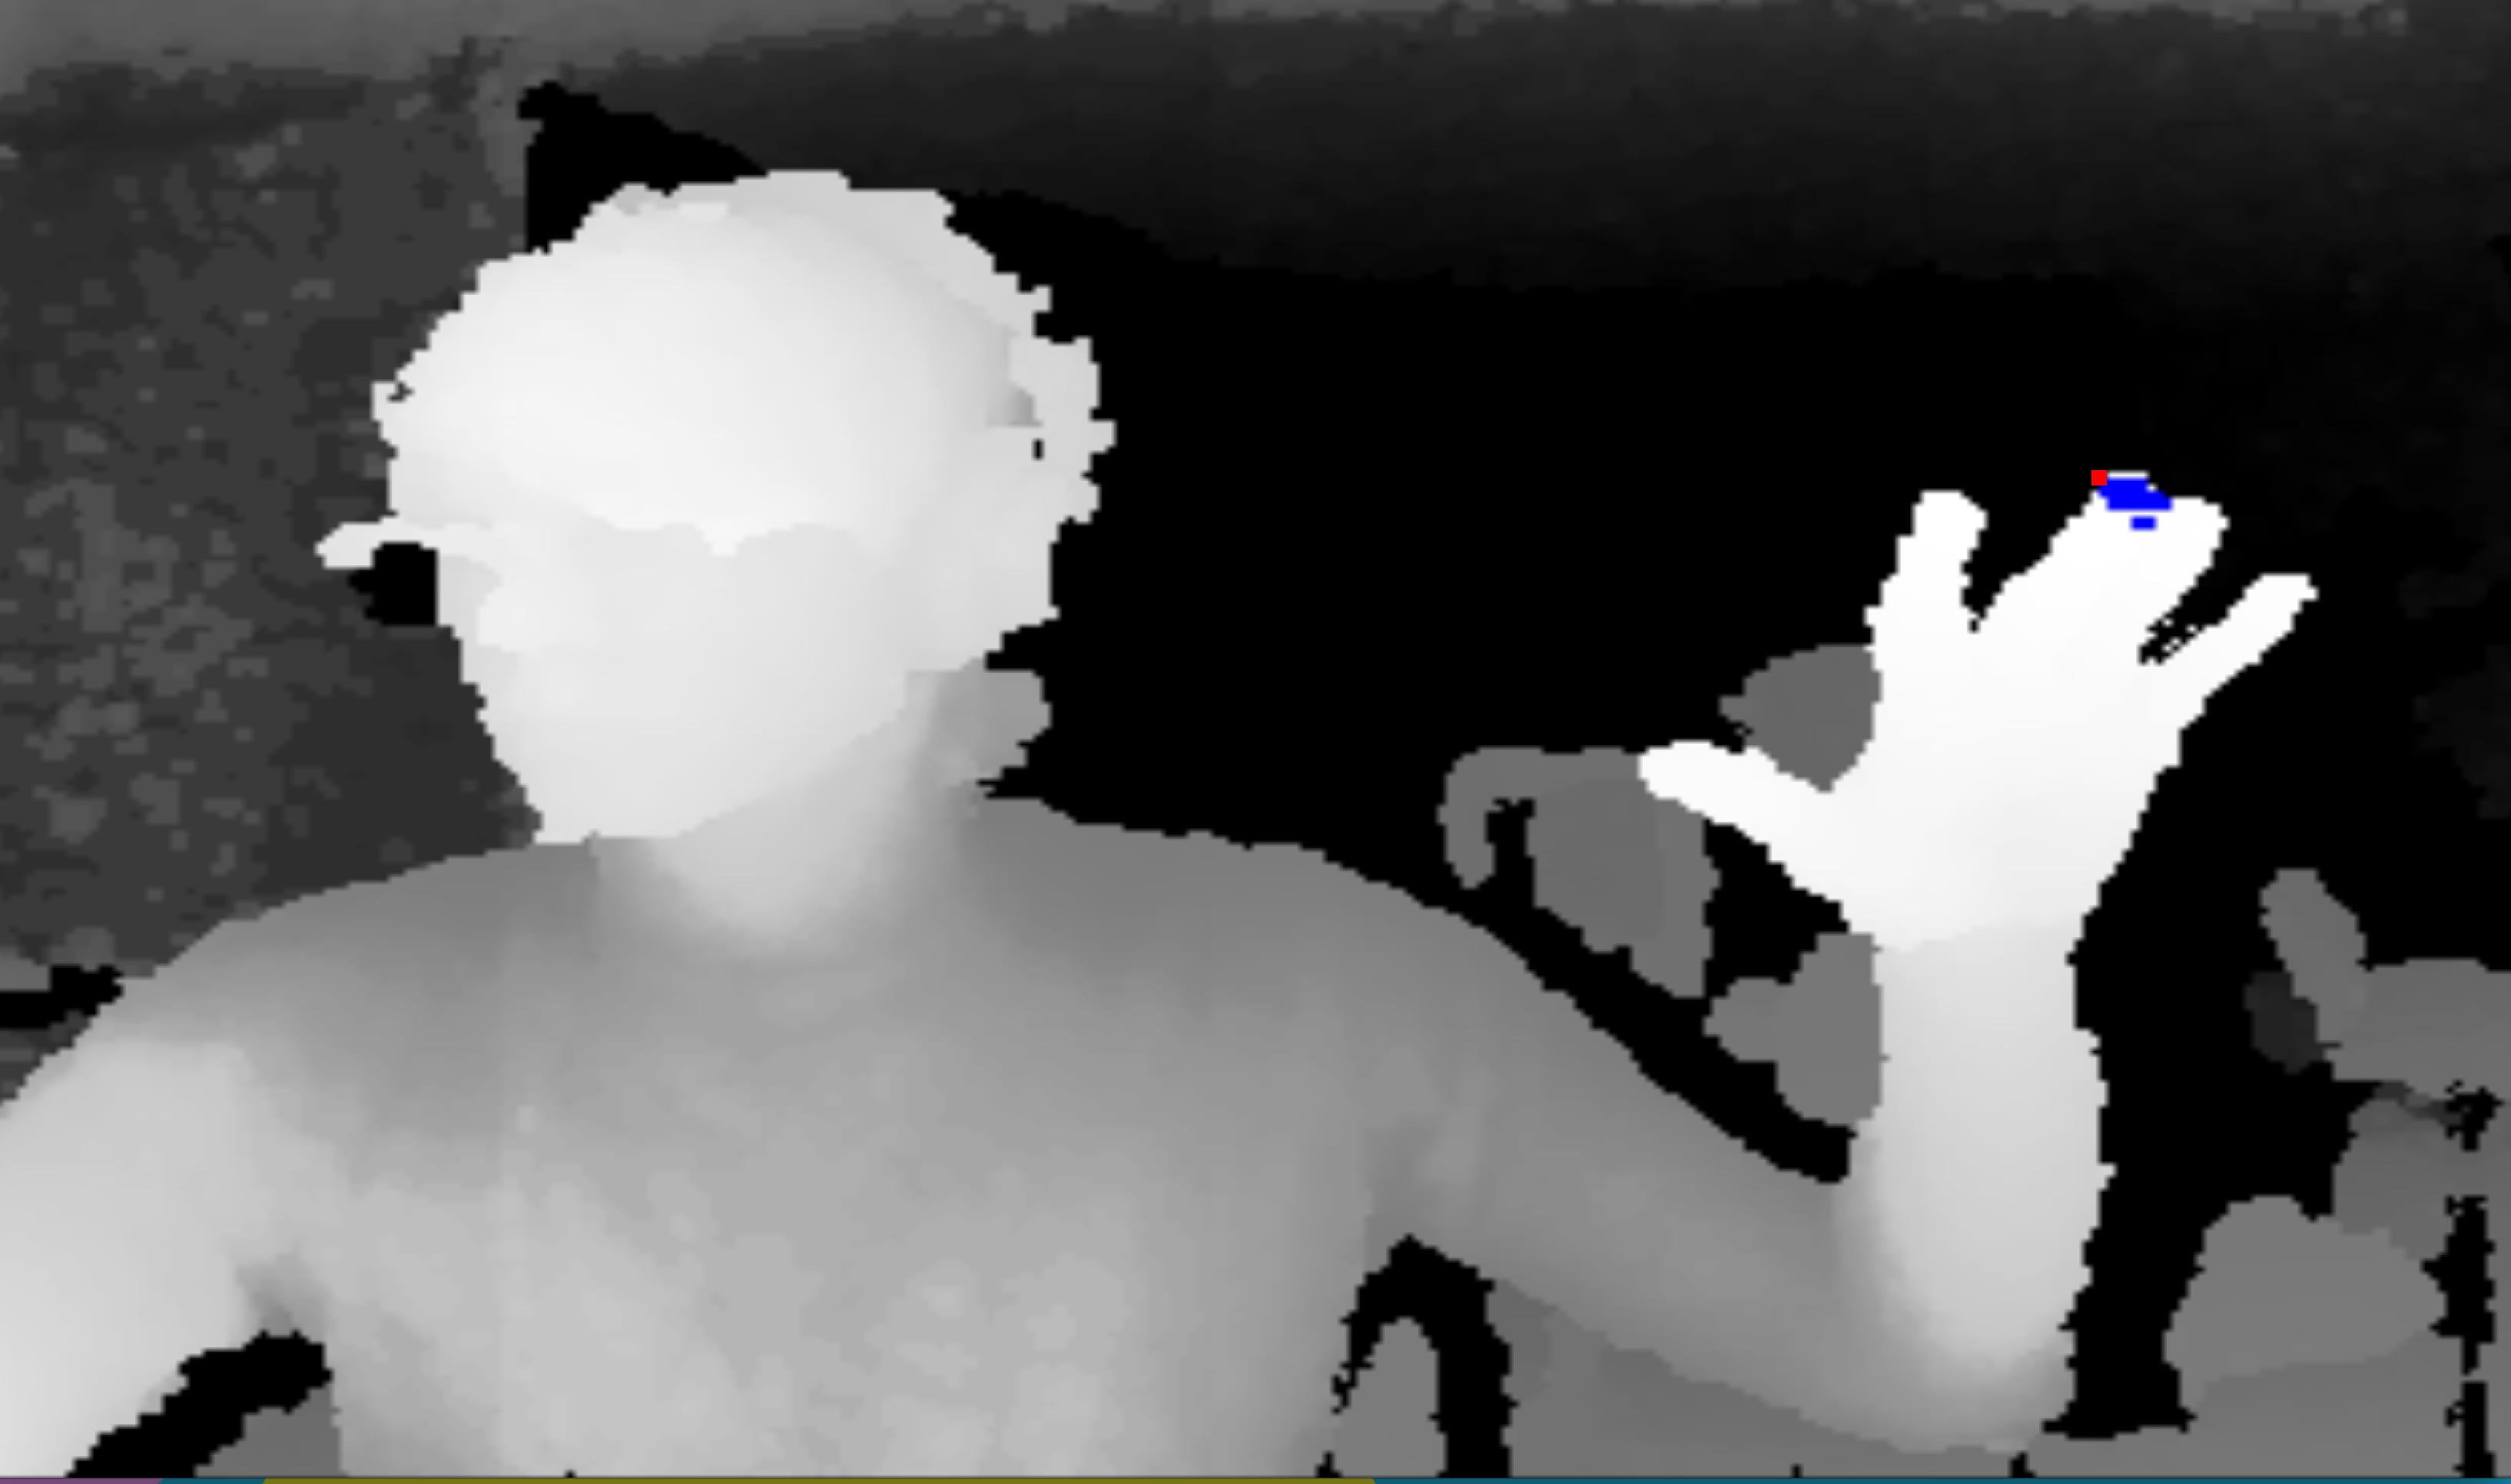
\includegraphics[width=0.8\linewidth]{depthimage}
  \caption{Depth image produced by a Depth Sensor.}
  \label{fig:depthimage}
\end{figure}

The Kinect version 1 uses a PrimeSense sensor which uses structured-light to
interpret depth, this works by projecting infrared points (IR) at the scene and
using an IR camera to interpret those points. The projected IR points have a
calibrated pattern which is picked up by the IR camera which is shown in figure
\ref{fig:ir}. All processing to determine depth from this IR image is done on
the sensor itself. 

\begin{figure}[h!]
  \centering
  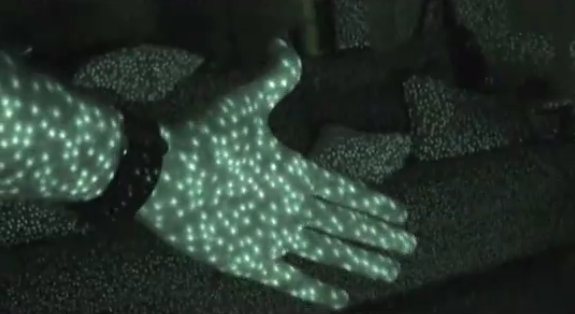
\includegraphics[width=0.8\linewidth]{KinectIR}
  \caption{Infrared light projected by the Kinect Sensor}
  \label{fig:ir}
\end{figure}


\subsection{Surface Measurement}
What we do in this step is that we take our depth image as described above and create a vertex map; this vertex map can be thought of as a point cloud or a collections of points as tuples $(x, y, z)$ in space, an example of this is shown in figure \ref{fig:pointcloud}. We also want to calculate the normal vectors for each of our given points as these normals help speed up some of the calculations we will wish to do later.

\begin{figure}
  \centering
  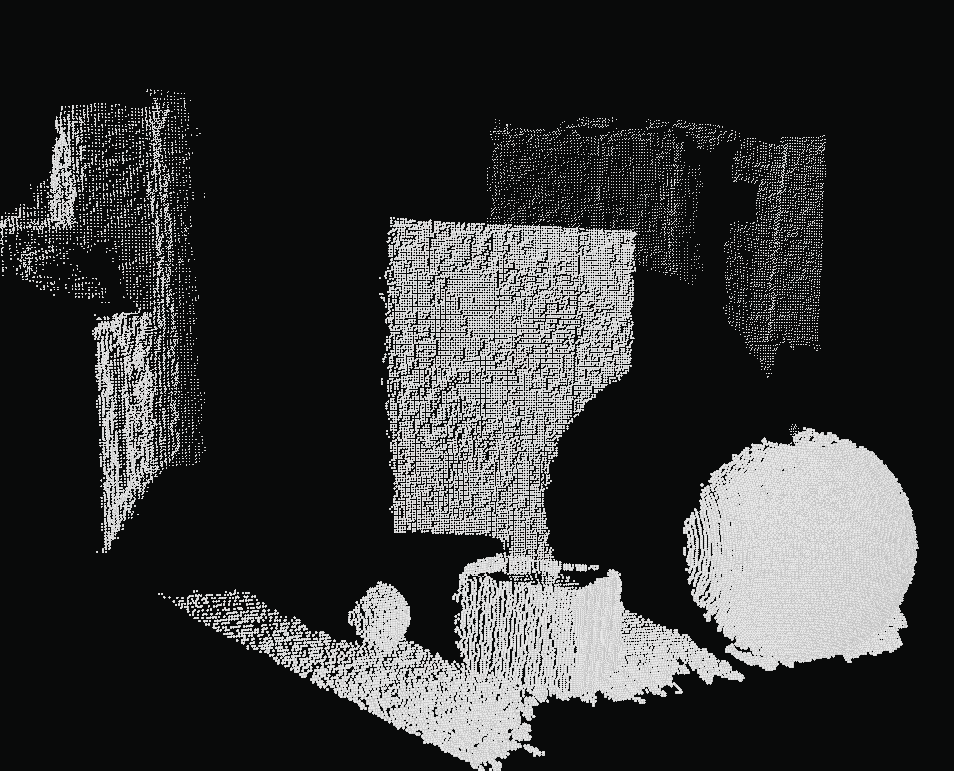
\includegraphics[width=0.8\linewidth]{pointcloud}
  \caption{Point cloud from a Kinect sensor.}
  \label{fig:pointcloud}
\end{figure}



At time $k$ raw depth map $R_k$---from the sensor---provides calibrated depth measurement $R_k(\mathbf{u}) \in \mathbb{R}$ at each image pixel $\mathbf{u} = (u,v)^{\top}$
A bilateral filter is applied $D_k(\mathbf{u})$ which will reduce noise in our depth image.
Filtered depth values are back projected into sensor frame of reference to obtain vertex map $\mathbf{V}_k$ where 

\begin{equation}
\mathbf{V}_k(\mathbf{u}) = D_k(\mathbf{u})\mathbf{K}^{-1}\dot{\mathbf{u}}
\end{equation}

where $\mathbf{K}$ is the constant calibration matrix inherent to the sensor and transforms points $\rightarrow$ image pixels, and the dot denotes homogeneous vectors $\mathbf{\dot{u}} := (\mathbf{u}^{\top}|1)^{\top}$
Since each frame is a measurment on a grid we can compute normal vectors with a cross product between neighboring map vertecies,

\begin{equation}
\mathbf{N}_k(\mathrm{u}) = v[(\mathbf{V}_k(u+1,v) - \mathbf{V}_k(u, v)) \times (\mathbf{V}_k(u,v+1) - \mathbf{V}_k(u,v))]
\end{equation}

 where $v[\mathbf{x}] = \mathbf{x} / \| \mathbf{x} \|_{2}$

We compute an $L = 3$ vertex and normal map pyramid, the first level of the
pyramid is the input depth map, we then down-sample this depth map to get the
second level then downsample once again to get the third level. 
Depth pyramid $D^{l \in[1\dots L]}$ bottom is original bilateral filtered depth map. 
At each level $\textbf{V}^{l \in[1\dots L]}$ $\textbf{N}^{l \in[1\dots L]}$ with the equations from the previous slide.
Given the camera $\rightarrow$ global co-ordinate frame transform $\mathsf{T}_{g,k}$, the global frame vertex is $\textbf{V}^{g}_{k} = \mathsf{T}_{g,k} \dot{\textbf{V}}_{k}(\mathrm{u})$
The equivalent mapping of normal vectors $\mathbf{N}^{g}_{k}(\mathbf{u}) = \mathsf{R}_{g,k}\mathbf{N}(\mathbf{u})$
This puts our vertex and normal maps into the global coordinate frame which is with respect to some $(0, 0, 0)$ (normally the location in which the scan was initiated).

\subsection{Fusion} \label{sec:fusion}
Each depth frame with its estimated pose, is fused into a single 3D
reconstruction using a volumentric truncated signed distance function. You can
think of this volume as a 3D grid that holds different values at each index. In
KinectFusion this volume is fixed as it is bound by GPU memory. 

The TSDF will be used to generate our mesh, we will also use the TSDF as a global reference for our new scans so that we can calculate the change in pose. 
A signed distance functions value corresponds to the closest zero crossing (surface interface), taking positive values from surface $\rightarrow$ free space, and negative values on the non-visible side. Figure \ref{fig:tsdfslice} shows how the TSDF can represent surfaces as zero crossings.
The TSDF is denoted by $\mathbf{S}_{k}(\mathbf{p})$ where $\mathbf{p} \in \mathbb{R}^{3}$ is a global frame point in the TSDF with a specified resolution. The continous TSDF will be denoted by $\mathbf{S}$

\begin{figure}
  \centering
  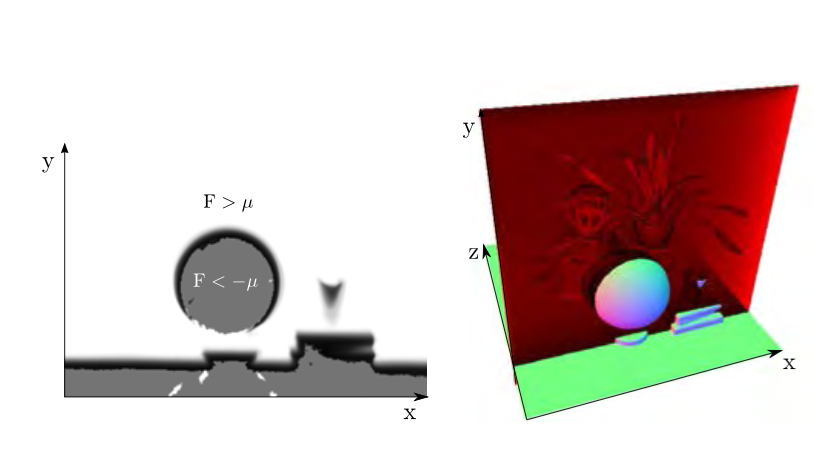
\includegraphics[width=0.8\linewidth]{tsdf}
  \caption{A slice of the truncated signed distance volume.}
  \label{fig:tsdfslice}
\end{figure}

Two Components are stored at each location of the TSDF: the current truncated signed distance value $\mathrm{F}_{k}(\mathbf{p})$ and a weight $\mathrm{W}_k(\mathbf{p})$.

\begin{equation}
\mathbf{S}_{k} \rightarrow [\mathrm{F}_{k}(\mathbf{p}), \mathrm{W}_{k}(\mathbf{p})]
\end{equation}

The TSDF is updated at an index $\mathbf{p}$ with,

\begin{equation}
\mathrm{F}_k(\mathbf{p}) = \frac{\mathrm{W}_{k-1}(\mathbf{p}) \mathrm{F}_{k-1}(\mathbf{p}) + \mathrm{W}_{\mathbf{R}_k}(\mathbf{p}) \mathrm{F}_{\mathbf{R}_k}(\mathbf{p})}{\mathrm{W}_{k-1}(\mathbf{p}) + \mathrm{W}_{\mathbf{R}_k}(\mathbf{p})}
\end{equation}

\begin{equation}
\mathrm{W}_k (\mathbf{p}) \leftarrow \mathrm{min} (\mathrm{W}_{k-1} (\mathbf{p}) + \mathrm{W} (\mathbf{p}), \mathrm{W}_{\eta})
\end{equation}

this updates the TSDFs distance value $\mathrm{F}_k$ and weight value $\mathrm{W}_k$ at the point $\mathbf{p}$ which updates our global model of the environments depth values and weight values. The weight $\mathrm{W}_k$ provides weighting of the TSDF proportional to the uncertainty of the surface measurement. It has been found that setting $\mathrm{W}_{\mathrm{R}_k} (\mathbf{p}) = 1$ resulting in a simple average, provides good results. 

\subsubsection{Surface Prediction from Ray Casting the TSDF} \label{sec:surface}
To estimate the change in pose, we must first create a vertex and normal map from the global TSDF by casting rays into the TSDF and finding zero crossings. This pointcloud that we predict is used to calculated the rigid body transform between the current camera pose and the global model.

We can compute a dense surface prediction by rendering the surface in a virtual camera with the current estimate $\mathsf{T}_{g,k}$. 
The surface prediction is stored as a vertex and normal map $\hat{\mathbf{V}}_{k}$ and $\hat{\mathbf{N}}_{k}$ and frame of reference $k$.
This is used in the subsequent camera pose estimation step.
In the global SDF, a per pixel raycast can be performed. Each ray $\mathsf{T}_{g,k}\mathbf{K}^{-1}\mathbf{\dot{u}}$ is marched starting from min depth for pixel and stopping at a zero crossing.
For points on or close to surface interface $F_{k}(\mathbf{p}) = 0$ we assume the gradient of the TSDF at $\mathbf{p}$ is orthogonal to the zero level set, so the surface normal for the associated pixel $\mathbf{u}$ can be computed directly from $F_{k}$ using a numerical derivative of the SDF:

\begin{equation}
\mathsf{R}_{g,k} \mathbf{\hat{N}}_{k} (\mathbf{u}) = \mathbf{\hat{N}}^{g}_{k} = v[\nabla F(\mathbf{p})], \nabla F = 
\begin{bmatrix}
    \frac{\delta F}{\delta x}, & \frac{\delta F}{\delta y}, & \frac{\delta F}{\delta z}
\end{bmatrix}^{\top}
\end{equation}

This provides us with an approximated vertex and normal map which is used in the sensor pose estimation step as the comparison previous vertex and normal map.


\subsubsection{Sensor Pose Estimation} \label{sec:pose}
Now that we have our vertex and normal map from our current frame and the global model we can estimated the change in pose for this frame. This will allow our new frame to be fused into the TSDF at the correct location.

The live 6DOF camera pose estimated for a frame at time k that is the rotation $\mathsf{R}_{g,k}$ and translation $\mathbf{t}_{g,k}$

\begin{equation}
\mathsf{T}_{g,k} = 
\begin{bmatrix}
  \mathsf{R}_{g,k} & \mathbf{t}_{g,k} \\
  0 & 1
\end{bmatrix}
\in \mathbb{SE}_{3}
\end{equation}

where $\mathbb{SE}_{3} := \{\mathsf{R}, \mathbf{t}\ |\ \mathsf{R} \in \mathbb{SO}_{3}, \mathbf{t} \in \mathbb{R}^{3}\}$

\hfill \break

To track the sensor frame, the live surface measurement $(\mathbf{V}_{k}, \mathbf{N}_{k})$ against the model prediction from the previous frame $(\mathbf{\hat{V}}_{k-1}, \mathbf{\hat{N}}_{k-1})$. First we must find correspondences between the two sets of points with projective data association. 


\begin{algorithm}
\caption{Projective point-plane data association.}\label{euclid}
\begin{algorithmic}[1]
\For{each image pixel $u \in$ depth map $\mathbf{D}_i$ \textbf{in parallel}}
\If {$\mathbf{D}_i(u) > 0$} 
\State $\mathbf{v}_{i-1} \leftarrow \mathbf{T}^{-1}_{i-1} \mathbf{v}^{g}_{i-1}$
\State $\mathbf{p} \leftarrow$ perspective project vertex $\mathbf{v}_{i-1}$
\If {$\mathbf{p} \in$ vertex map $\mathbf{V}_i$}
\State $\mathbf{v} \leftarrow \mathbf{T}_i \mathbf{V}_i(p)$
\State $\mathbf{n} \leftarrow \mathbf{R}_i \mathbf{N}_i(p)$
\If {$\|\mathbf{v} - \mathbf{v}^{g}_{i-1} \| <$ distance threshold and $abs(\mathbf{n} \cdot \mathbf{n}^{g}_{i-1}) <$ normal threshold}
\State point correspondence found
\EndIf
\EndIf
\EndIf
\EndFor
\end{algorithmic}
\end{algorithm}


Given these correspondences the output of each ICP iteration is a single transformation matrix $T$ which minimizes the point to plane error metric, or the sum of squared distances between each point in the current frame and the tangent plane at corresponding points in the previous frame. Figure \ref{fig:pointplane} \cite{Low04linearleast-squares} provides a visual explanation of how this point to plane error metric works in 2D.

\begin{equation}
\mathbf{E}(\mathsf{T}_{g,k}) = 
\sum_{\substack{
   \mathbf{u} \in \mathcal{U} \\
   \Omega_{k}(\mathbf{u}) \neq null
  }}
  \| ( \mathsf{T}_{g,k} \mathbf{\dot{V}} (\mathbf{u}) - \mathbf{\hat{V}}^{g}_{k-1} (\mathbf{\hat{u}}))^{\top} \mathbf{\hat{N}}^{g}_{k-1} (\mathbf{\hat{u}}) \|_{2}
\end{equation}


A linear approximation is used to solve this system, we assume that the transformation between two frames is incremental.

\begin{figure}
  \centering
  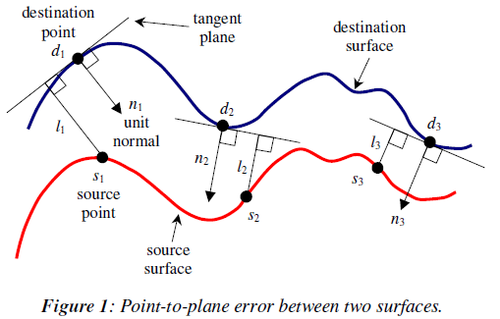
\includegraphics[width=1.0\linewidth]{pointplane}
  \caption{Point-to-plane error between two surfaces.}
  \label{fig:pointplane}
\end{figure}

\subsubsection{System Overview}
Now that we have seen how each system works separately it helps to see how each
piece works together to make this system work as well as it does. Figure
\ref{fig:workflow} shows how each output from each calculation we have made is
used in the system. 

To summarize, the input image $\mathsf{R}_k$ is passed to
the surface measurement component and the component that updates our current
reconstruction. From the measurement we pass our surface vertex and normal maps
$\mathbf{V}_k$ and $\mathbf{N}_k$ to the pose estimation component, this
requires our predicted vertex and normal maps as we
must calculate the transform with respect to our model. The pose we calculated
is sent to the reconstruction updating component where the frame $\mathsf{R}_k$
is integrated into our Global TSDF, in the prediction phase we raycast our
current TSDF to come up with our predicted vertex and normal maps. This process
is fast enough for this system to run at 30 frames per second. Figure
\ref{fig:visworkflow} shows a more visual overview of this system.

\begin{figure}
  \centering
  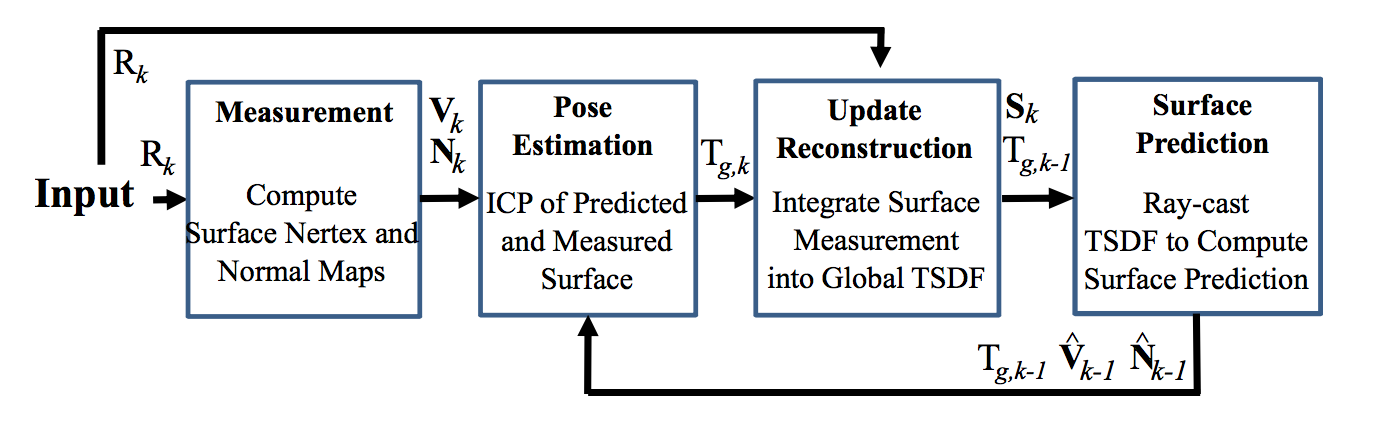
\includegraphics[width=1.0\linewidth]{workflow}
  \caption{Overview of the KinectFusion system.}
  \label{fig:workflow}
\end{figure}

\begin{figure}
  \centering
  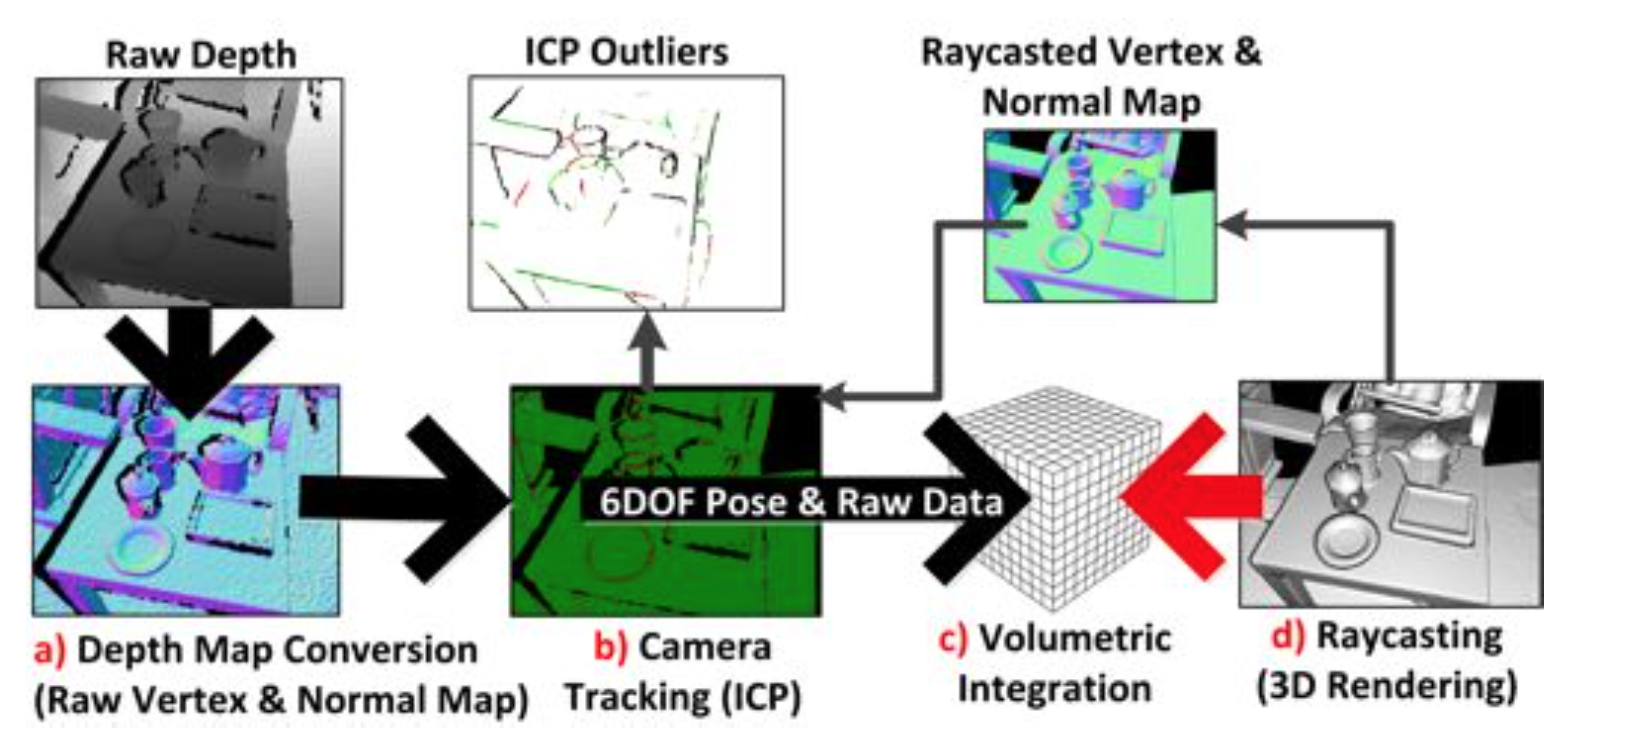
\includegraphics[width=1.0\linewidth]{kinectfusion}
  \caption{Overview of the KinectFusion system.}
  \label{fig:visworkflow}
\end{figure}



\section{VoxelHashing}
Now we will cover the novel aspects presented by Nie{\ss}ner et. al
\cite{niessner2013hashing}. In this section the pipeline and novel data structure used for
scanning and storing the scene will be explained. 

This data structure allows for the following main features: 

\begin{itemize}
    \item Efficient compression of volumetric TSDFs, maintaining resolution.
    \item Fusing new samples into the hash table
    \item Removal and garbage collection of voxel blocks, without reorganizing
        the data structure.
    \item Easy streaming of voxel blocks between the host and GPU memory, for
      large scale scans.
    \item Extraction of isosurface (mesh) using standard raycasting
        operations, for rendering and camera pose tracking.
\end{itemize}


\subsection{Pipeline}

Central to the overall architecture of this paper is a hash table data structure
that stores sub-blocks containing TSDFs, called voxel blocks. At each voxel a
value, weight, and color are stored. The hash table itself is not organized
spatially---neighboring voxel entries are not actually neigboring each other in space.

\begin{figure}
  \centering
  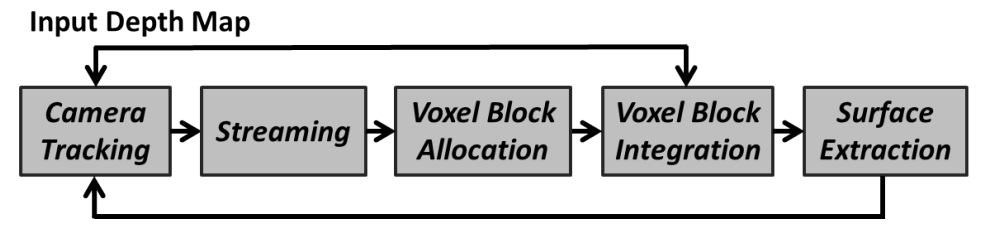
\includegraphics[width=1.0\linewidth]{voxelhashingpipeline}
  \caption{Voxel hashing pipeline.}
  \label{fig:vhpipeline}
\end{figure}


The system starts by reading a new input from the depth camera, and fusion---also
reffered to as integration---is performed. Voxel blocks in the view frustum are
allocated based on the input depth map. Only occupied voxels are allocated, and
empty space is ignored. The allocated voxel blocks are updated with the input
depth map---color, weight and value are each updated. Voxel blocks too far from
the scanned surface are garbage collected---removed from the hash table freeing
the allocated memory. This ensures that the data structure remains sparse over
time. After integration, the surface is raycasted from the current estimated
camera pose. This extracted information is passed back to camera tracking to
estimate the camera's 6DoF pose using Iterative Closest Points. The system also
performs bidirectional streaming between GPU and host memory, which allows
previously scanned voxel blocks to be streamed back to the GPU for further
updates. The entire process is shown visually in figure \ref{fig:vhpipeline}.

\subsection{Data Structure}
Figure \ref{fig:hashtable} shows the voxel hashing data structure. One way to think
about this data structure is that an infinite uniform grid subdivides the world
into voxel blocks. Each block is a regular voxel grid. In this implementation
the voxel block consists of $8^3$ voxels where each voxel stores a TSDF value, color
and a weight. This structure is shown visually in figure \ref{fig:hashtable}.

\begin{figure}
  \centering
  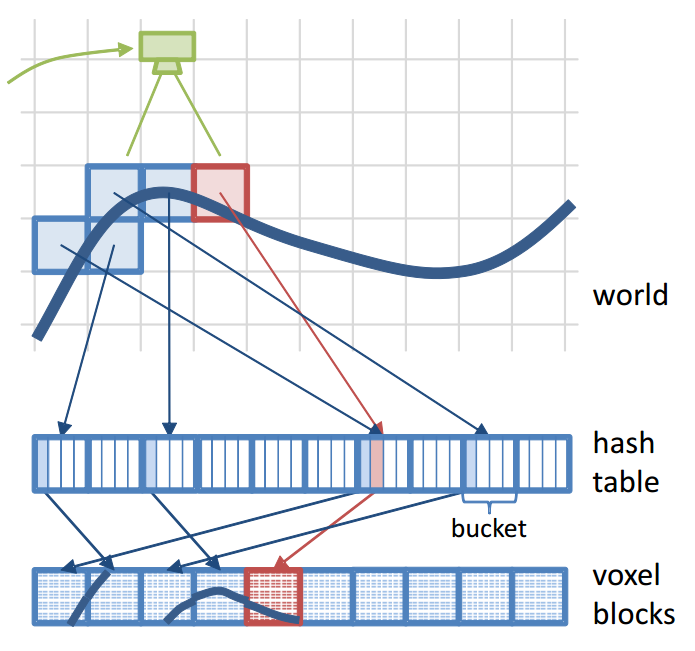
\includegraphics[width=1.0\linewidth]{hashtable}
  \caption{Visualization of the table.}
  \label{fig:hashtable}
\end{figure}

%todo ? add voxel struct

To exploit sparsity of environments---the fact that most environments are
empty space---voxel blocks are only allocated around surface geometry. A GPU
accelerated hash table is used to manage allocation and retrieval of voxel
blocks. The hash table stores hash entries which have a pointer to a voxel block
in GPU memory. These blocks can be retrieved using the world coordinates of the
voxel block $(x,y,z)$; These coordinates are rounded. The world coordinate is
mapped to a hash value $H(x,y,z)$ using the hash function below:
\begin{equation}
  H(x,y,z) = (x * p_1 \oplus y * p_2 \oplus z * p_3) \mod n
\end{equation}
Where $p_1$, $p_2$, and $p_3$ are large primes (in the case of this papere 73856093,
19349669, 83492791 respectively based on Teschner et al.) and n is the hash
table size. 

% todo ? add hash entry struct

\subsubsection{Resolving Collisiions}
Collisions in the hash table will occur when different allocated blocks map to
the same hash value. These collisions are handled by creating buckets in the
hash table that map to one unique hash value. Each bucket stores a number of
hash entries. When there is a collision the current hash entry is stored in the
next available entry in the bucket. If the bucket is full---which will rarely
happen with a reasonable table and bucket size---a linked list entry is appended
filling spots in the subsequent buckets. These linked list entries are stored in
the offset pointer in the hash entry. In general the last entry in a bucket will
be the head of the linked list.

\subsubsection{Hashing Operations}

\noindent
\textbf{Insertion} to insert a hash entry, the hash function is evaluated which
maps to a bucket. We linearly search through the bucket to find an empty space
and if needed the linked list to find a position to store the new entry. To
avoid race conditions the bucket is locked during insertion. 

\noindent
\textbf{Retrieval} To read a value from the hash table the hash function is
evaluated and perform a linear search through the bucket and the attached linked
list if it exists. The search does not stop at empty entries as removing values
can leave the bucket fragmented.

\noindent
\textbf{Removal} The hash function is evaluated for a given world coordinate and
linearly search the corresponding bucket, traversing the linked list if needed.
If we find a match to the given entry without traversing the list we can just
delete the entry. However if the list was traversed we must ensure that we
update the linked list. If the hash entry we wish to delete is a linked list
head---it is the last element in the bucket---then the hash entry pointed to by
that offset is copied into the last element of the bucket. Otherwise the element
is not the head and can be removed, updating the linked list pointers. If the
linked list is updated we must lock the bucket atomically.

\begin{figure}
  \centering
  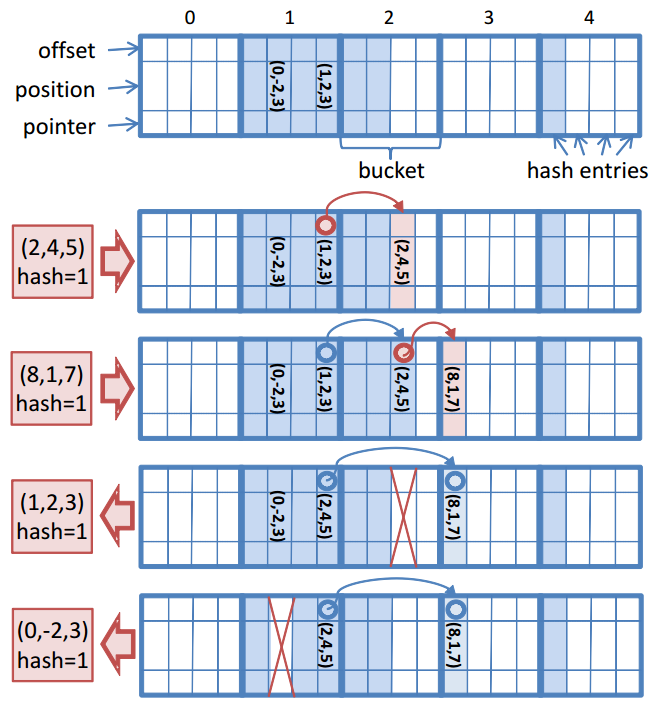
\includegraphics[width=1.0\linewidth]{hashtableoperations}
  \caption{Hash table operations showing insertion and removal of values that
    all map to a hash value of 1.}
  \label{fig:hashingoperations}
\end{figure}


\subsection{Voxel Block Allocation}
Prior to integration of new TSDFs, corresponding voxel blocks that are within
the bounds of the depth sample must be allocated in the hash table. 

For each input depth sample a ray is created with an interval bound to the
truncation region of the observed surface. For each candidate found, a new voxel
entry is added to the hash table. This ray based approach provides much better
performance than modeling the entire view frustum and provides sufficient
coverage of the scene to be scanned.

Once the blocks have been inserted, GPU memory is allocated for the voxel block
data. The memory on the GPU is divided into blocks. The blocks are managed by a
list of available blocks, which is a linear buffer with indices pointing to
unallocated blocks. This list must be updated atomically and is updated on
insertion and removal. The last index in the list is used for a new block allocation.

\subsection{Voxel Block Integration}

Integration (fusion) is very similar to the previous implementation from Kinect Fusion
mentioned in \ref{sec:fusion}. The important difference is how the voxel blocks
are selected.

\noindent
\textbf{Voxel Block Selection} Voxel blocks are selected for integration by
first, in parallel, accessing all the hash table entries storing a binary flag.
1 for occupied visible blocks and 0 otherwise. This array is scanned with a
parallel prefix sum \cite{harris2007parallel}. The hash table can be arbitrarily
large so a three level up and down sweep is used. Using these results a compact
hash table is created in a different buffer, containing all blocks within the
view frustum (see \ref{fig:selection}).

\begin{figure}
  \centering
  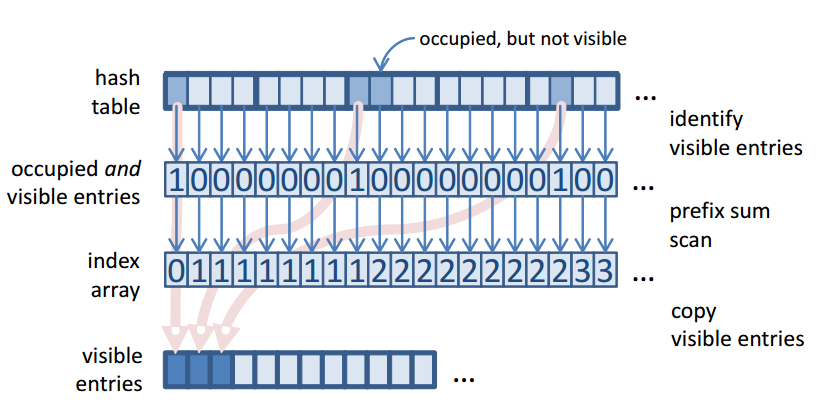
\includegraphics[width=1.0\linewidth]{viewfrustumselection}
  \caption{Voxel block selection for updates.}
  \label{fig:selection}
\end{figure}

\noindent
\textbf{Surface Update} The list of hash entries that were generated is
processed in parallel to update the TSDF values. One GPGPU kernel is executed
for each block, and one thread is allocated per voxel.

Updating the voxel blocks requires computing the associated TSDFs, both weights
and colors. Depth values are integrated using a a running averages as in Curless
and Levoy \cite{curless1996}. 

The weights are set according to the depth values, this allows the the noise of
the sensor to be incorperated. Near values are given a higher weight than those
further away as those closer are assumed to be less noisy. 


\subsection{Surface Extraction}

Surface extraction is performed in the same way as described in section \ref{sec:surface}.

\noindent
\textbf{Camera Tracking} After we have extracted the surface via raycasting, it
can be shaded and displayed to the users, and used for frame-to-model camera
pose estimation \cite{newcombe11}. The next input frame from the depth camera is
used with the raycasted depth map to estimate pose, this is exactly the same as
the process detailed in section \ref{sec:pose}.


\subsection{Streaming}
To allow for unbounded reconstructions a bidirectional GPU-Host memory streaming
scheme is used. 

This unstructured data structure makes this process trivial as there is no
reorganization required as in the heirarchical approach. An active region is
defined as a sphere containing the view frustum and some padding around it. This
streaming occures at every frame just after camera pose estimation. This is
shown in figure \ref{fig:streaming}.

\subsubsection{GPU-to-Host}
Streaming from the GPU to the host requires looking through the hash table and
marking voxel blocks which will be outside of the active region. These voxel
blocks are deleted from the data structure on the GPU and added to an
intermediate buffer. 

In host memory the data is no longer stored in a hash table, rather the world
space is divided into chunks (in their implementation $1m^3$). Voxel blocks are
added to these chunks and a descriptor for hash entry information is added to
each voxel block.

\subsubsection{Host-to-GPU}
To move from host to GPU chunks that fall entirely into the active region must
be identified. Host-to-GPU streaming is executed on a per chunk basis rather
than per voxel as with GPU-to-Host. 

For performance, streaming host-to-GPU is limited to one chunk per frame. Once
selected, the chunk is streamed to the intermediate buffer created for
GPU-to-Host streaming. The voxel blocks now in the intermediate buffer are
reinserted into the hash table using the voxel block descriptors. Reallocating
memory on the heap for these voxel blocks and copying them to their respective
locations. 

\begin{figure}
  \centering
  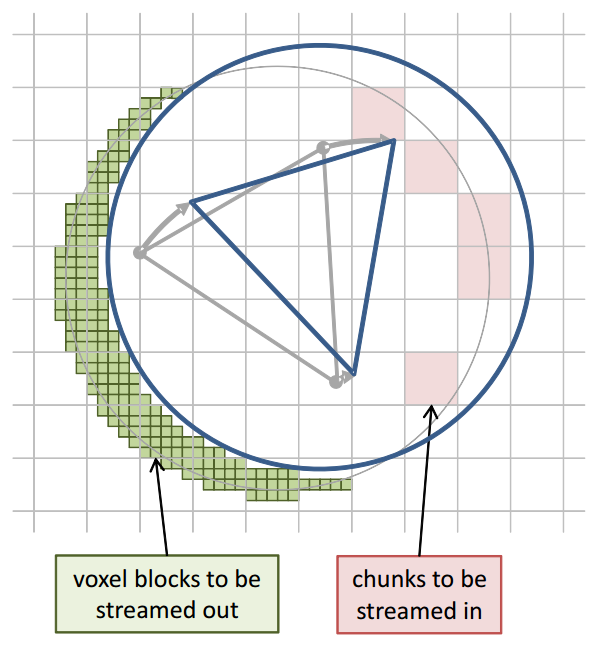
\includegraphics[width=1.0\linewidth]{streaming}
  \caption{Camera moving from left to right. Voxel blocks leaving the camera
    frustum are streamed out (green). Streaming in happens in chucks (red blocks).}
  \label{fig:streaming}
\end{figure}



\subsection{Results}
Comparisons of voxel hashing to other similar systems are shown in 
figure \ref{fig:comparetracking}. Comparisons with other moving volume approaches were
conducted. First a comparison with Extended Fusion \cite{Whelan14} \cite{roth2012moving} which uses a
uniform regular grid that moves through the environment streaming data out as an
optimized mesh. Second, a comparison to Heirarchical Fusion
\cite{chen2013scalable} which supports larger moving volumes.

Shown in figure \ref{fig:compare}, the quality and scale of the reconstruction
with the voxel hashing approach is greater than other approaches. Figure
\ref{fig:framerate} shows a comparison of the framerates of the different systems.


\begin{figure}
  \centering
  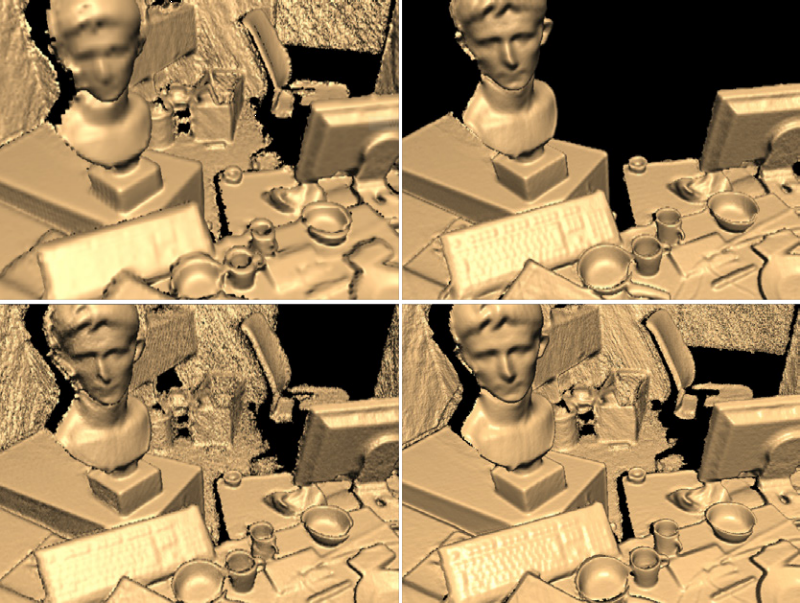
\includegraphics[width=1.0\linewidth]{comparison}
  \caption{Quality and scale comparison between similar systems. Bottom right:
    Voxel hashing at 4mm voxel size. Top: Moving volumes (top right) at the same
    resolution, (top left) reduced resolution for equivalent scale. Bottom Left:
    hierarchical grids approach.}
  \label{fig:compare}
\end{figure}

\begin{figure}
  \centering
  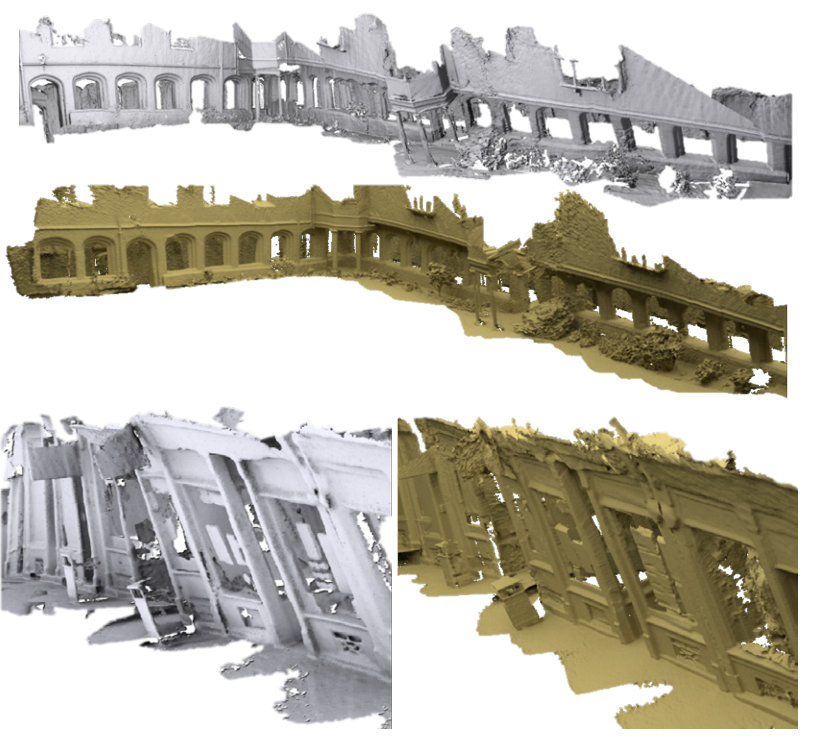
\includegraphics[width=1.0\linewidth]{compare}
  \caption{Comparison of the tracking drift. In grey is the hierarchical
    approach of Chen et al. \cite{chen2013scalable} and in yellow is the results
  from this paper.}
  \label{fig:comparetracking}
\end{figure}


\begin{figure}
  \centering
  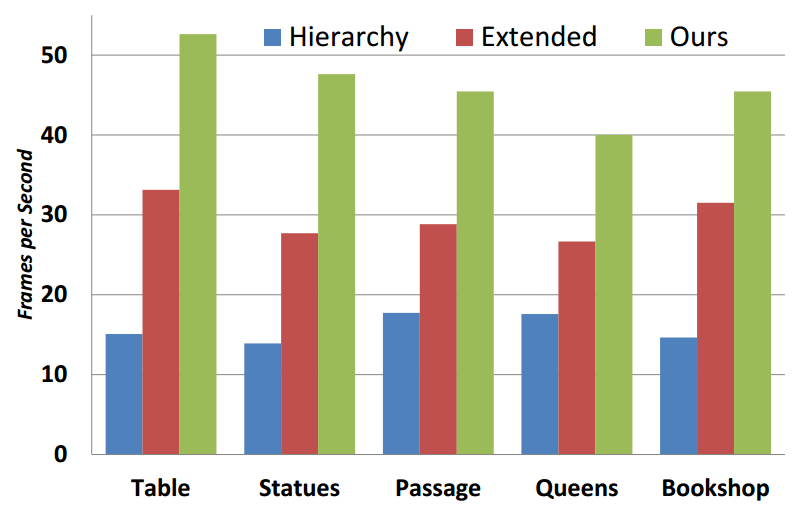
\includegraphics[width=1.0\linewidth]{results}
  \caption{Framerate comparison between the different approaches.}
  \label{fig:framerate}
\end{figure}


\section{Open Source Implementations} \label{sec:opensource}
There are a few open source implementations of the KinectFusion system and its
extensions:
\begin{enumerate}
  \item Microsoft KinectFusion \cite{MSKinectFusion}
  \item KFusion \cite{kfusion}
  \item KinFu from Point Cloud Library (PCL) \cite{kinfu}
  \item RXKinFu a fork of PCL KinFu from Northeastern University \cite{RXKinFu}
  \item VoxelHashing source code (this paper) \cite{voxelhashing}
  \item InfiniTAM a framework for Volumetric Fusion of depth images \cite{prisacariu2014}
\end{enumerate}

 I have tested many of the different implementations of these systems. 
Many of the moving volume implementations have issues with tracking as
 described above. The implementations of Voxel Hashing however are much better
 at tracking, scale, and speed.

\subsection{KinectFusion Implementations}
\subsubsection{Microsoft KinectFusion}
This implementation has partial code availability it comes with the new Kinect SDK, it is limited to a fixed volume. It is not fully open-source as some of the headers access closed source libraries that implement many of the important functions that comprise the system. 

\subsubsection{KFusion}
KFusion is an implementation of the initial KinectFusion algorithm based on the
paper by Newcombe et al. \cite{newcombe11} and Izadi et al. \cite{izadi11}. It is a standalone application with a very simple structure that is helpful to understand each individual part of the system.

\subsubsection{KinFu}
KinFu is a fully open source implementation from the Point Cloud Library team,
there are 2 implementations available a fixed volume version KinFu and a large
scale version KinFu Large Scale which uses moving volumes to extend its volume.

\subsubsection{RXKinFu}
This is a standalone fork of KinFu and provides the extended volume features
presented by Roth et al. \cite{roth2012moving}. 

\subsection{VoxelHashing Implementations}
\subsubsection{VoxelHashing}
Implementation of the system presented in this paper \cite{niessner2013hashing}.

\subsubsection{InfiniTAM}
This implementation provides multiple different approaches for volumetric fusion
based on your application. It includes implementations of both the original
KinectFusion implementation \cite{newcombe11} \cite{izadi11} and VoxelHashing \cite{niessner2013hashing}.


\section{Reflections on My Presentation}
My presentation was a bit rushed as this paper requires and understanding of
much of the previous work and a lot of content needed to be covered in a short
time. 
I really need to learn to slow down when I am presenting and allow different ideas to
sink in for the audience. Conceptualy the paper seemed to be understood---at
least what it was trying to achieve---as the questions I recieved were
applicability regaurding different situations. This is a fairly complex paper that
requires knowledge of GPGPU computing, general graphics, data structures, and
some involved algorithms; however I think that exposing people to these sorts of
high performance computing and parallel ideas is important as applications get
faster and more complex. I think think the presentation was at an adequate level
but for the time alloted it may have been a bit more than I was able to explain
effectively. 

\bibliographystyle{abbrv}
\bibliography{reconstruction}


%\includegraphics[width=1.0\linewidth]{algorithm2}
%\includegraphics[width=1.0\linewidth]{algorithm3}

\end{document}
